\chapter{Aufgaben}
Bei den Aufgaben werden mit LTSpice Schaltungen zusammengestellt, welche dann praktisch im Labor nachgebaut werden können. In den folgenden Aufgaben werden verschiedene Schaltungen wie Signalquellen, Spannungsteiler und Potentiometer zusammengestellt. 

\section{Signalquellen}
Hier ist der Aufbau einer einfachen Signalquelle zu sehen, welche eine Spannung von 1V besitzt.
\begin{figure}[h!]
\centering
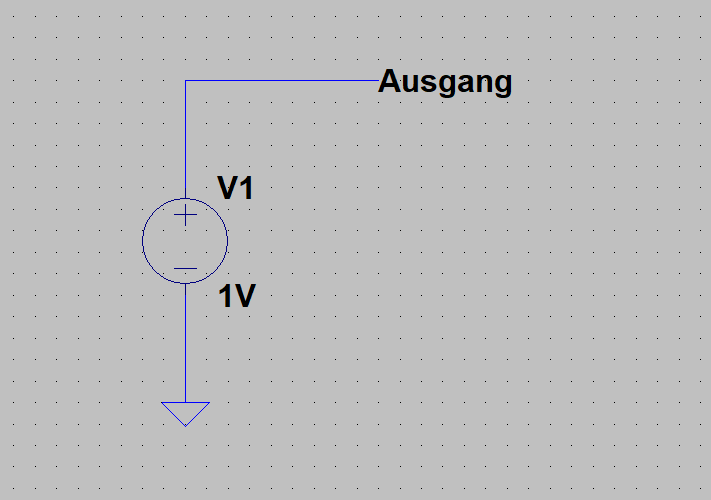
\includegraphics[scale=1]{21.PNG}
\caption{Darstellung einer Signalquelle in LTSpice}
\label{fig: Signalquelle}
\end{figure}
\newpage
Im Folgenden werden mit der Schaltung \fref{fig: Signalquelle}, verschieden Kurvenformen dargestellt und mit den jeweiligen Werten in LTSpice simuliert:



\subsection{Gleichspannungsquelle}
Folgender LTSpice Simulation und Graph wird durch eine Gleichspannungsquelle erzeugt.
\begin{figure}[ht!]
\centering
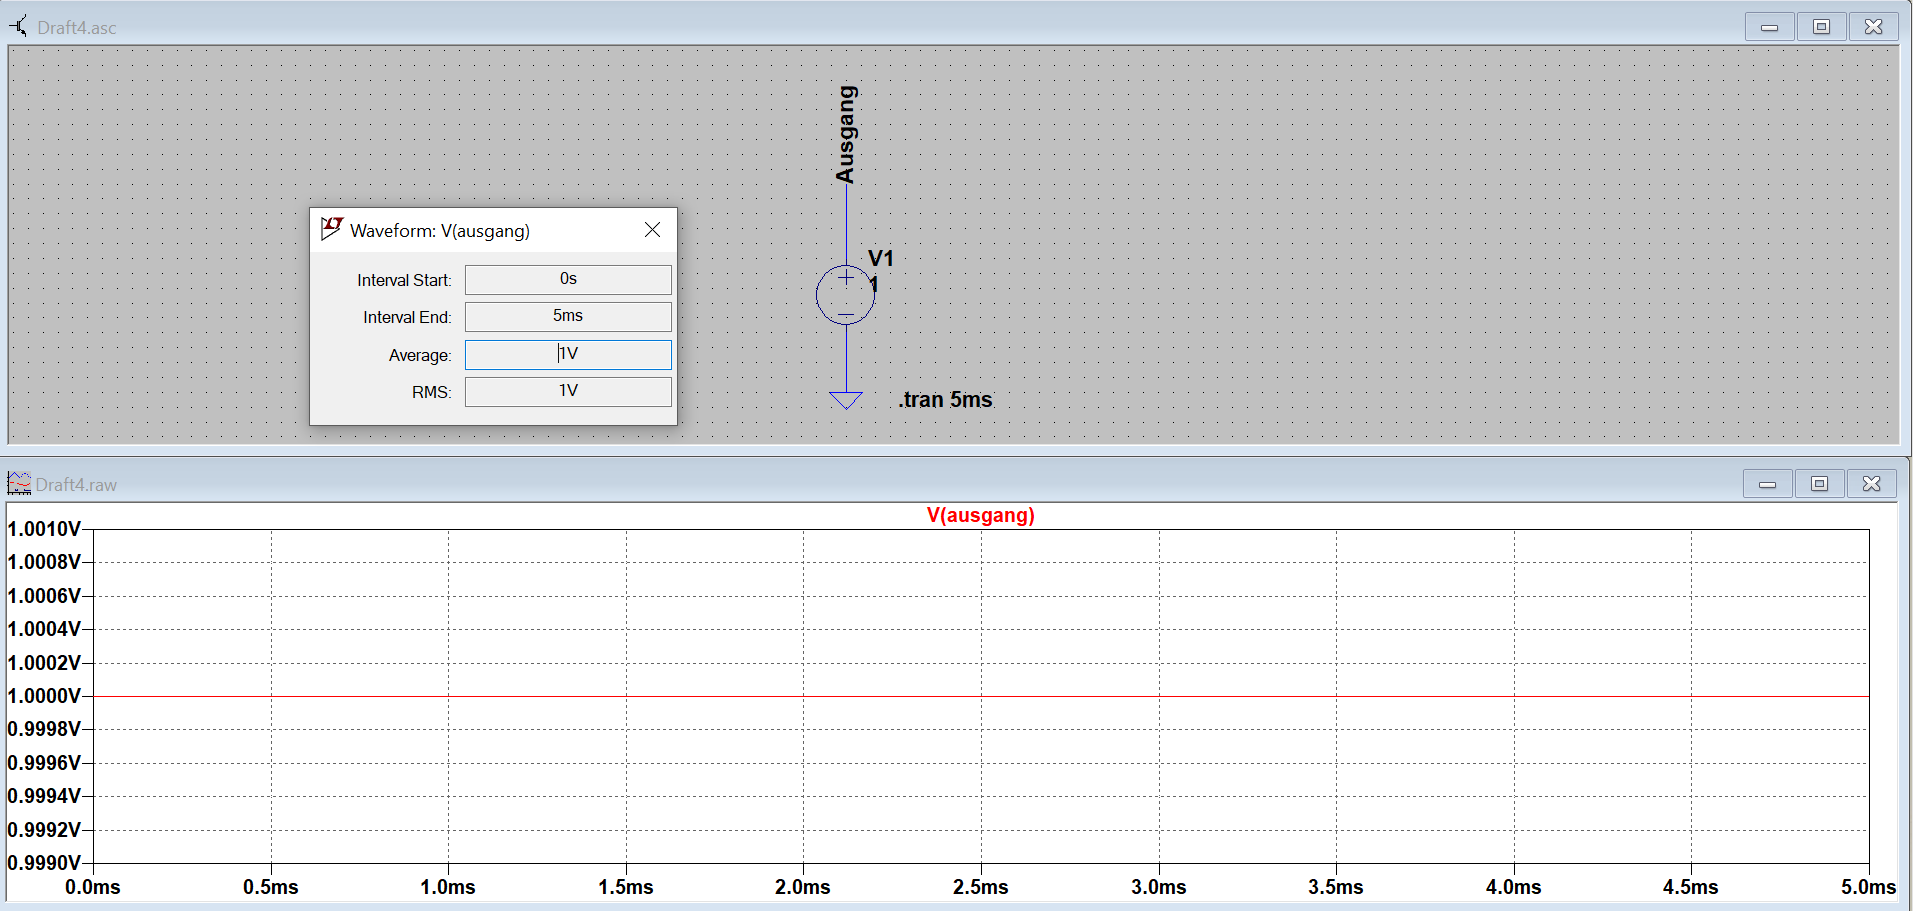
\includegraphics[scale=0.5]{211.PNG}
\caption{Gleichspannungsquelle $U=1V$}
\end{figure}

\subsection{Signussignal}
Um bei der folgenden Simulation ein richtiges Signal heraus zu bekommen, muss die $Periode(T)=1ms$ in die Frequenz f umgerechnet werden.
\begin{equation}
f=\frac{1}{T}=\frac{1}{10^{-3}}=1000Hz
\end{equation}
Folgender LTSpice Simulation und Graph wird durch die Werte erzeugt.
\begin{figure}[h!]
\centering
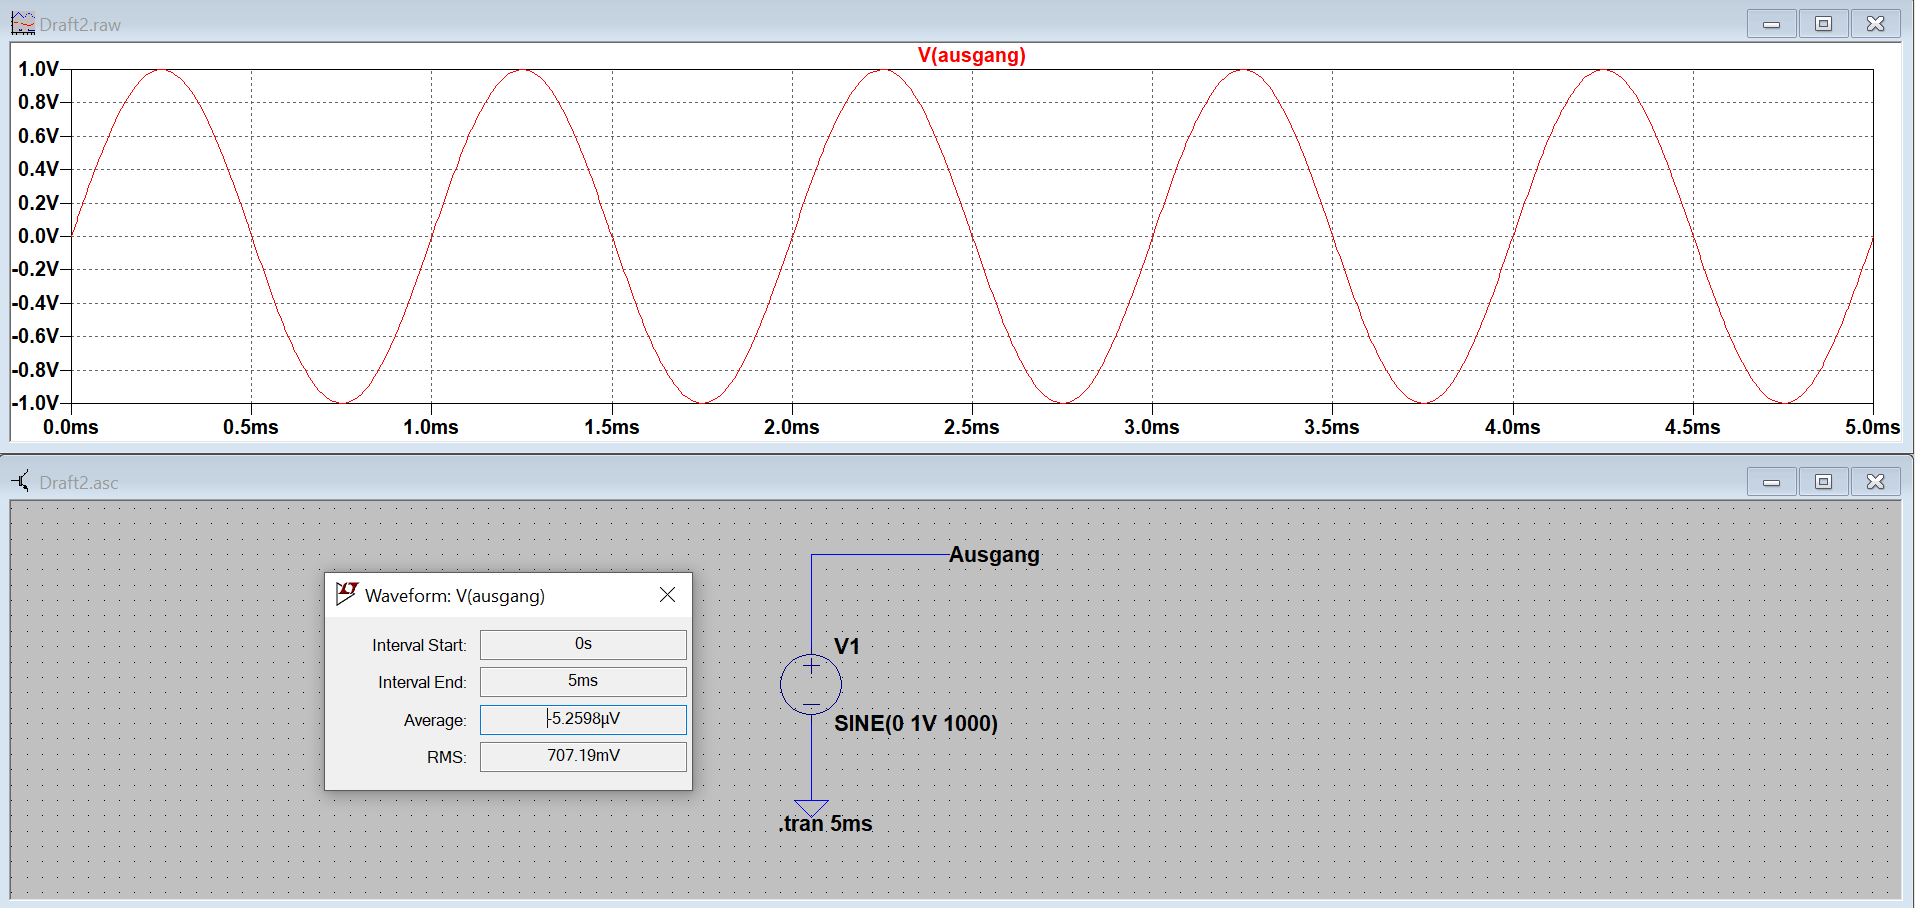
\includegraphics[scale=0.5]{212.PNG}
\caption{Sinussignal mit $\^{U}=1V$ und $T=1ms$}
\label{fig: Sinussignal}
\end{figure}
\newpage

\subsection{Symmetrisches Rechtecksignal}
Zum Darstellen eines symmetrischen Recktecksignals wird der $T_{rise}$ und $T_{fall}$ Wert angepasst. Dieser liegt in der Simulation bei jeweils 1ns. Die Spannungsquelle wird in den Pulse-Mode gestellt und die Werte für $\^{U}$,$T_{on}$ und f eingetragen \fref{fig: symRechtecksignal}. Dabei ergibt sich folgende LTSpice Simulation und Graph. 
\begin{figure}[ht!]
\centering
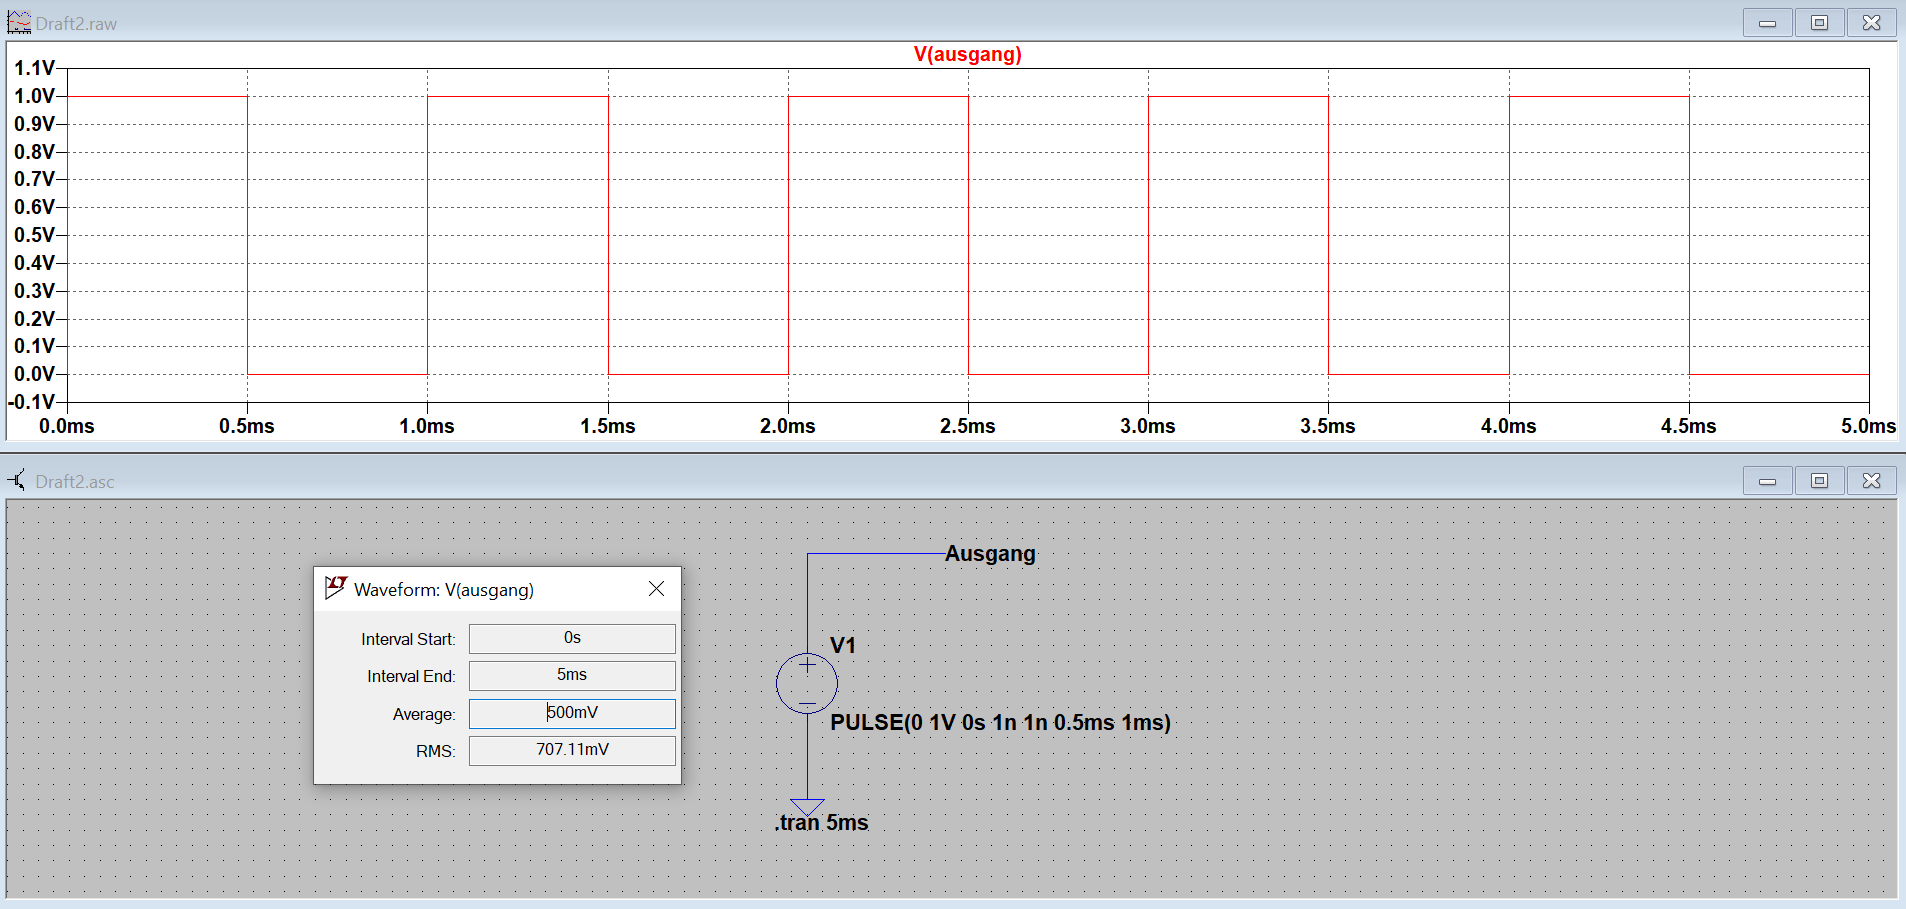
\includegraphics[scale=0.5]{213.PNG}
\caption{Symmetrisches Rechtecksignal mit $\^{U}=1V$, $T_{on}=0,5 ms$ und $f=1ms$}
\label{fig: symRechtecksignal}
\end{figure}

\subsection{Unsymmetrisches Rechtecksignal}
Zum Darstellen eines unsymmetrischen Recktecksignals wird ebenfalls der $T_{rise}$ und $T_{fall}$ Wert angepasst. Der liegt bei dieser Simulation bei jeweils 1ns. Durch eintragen der restlichen Werte \fref{fig: unsymRechtecksignal}, ergibt sich folgende LTSpice Simulation und Graph.
\begin{figure}[ht!]
\centering
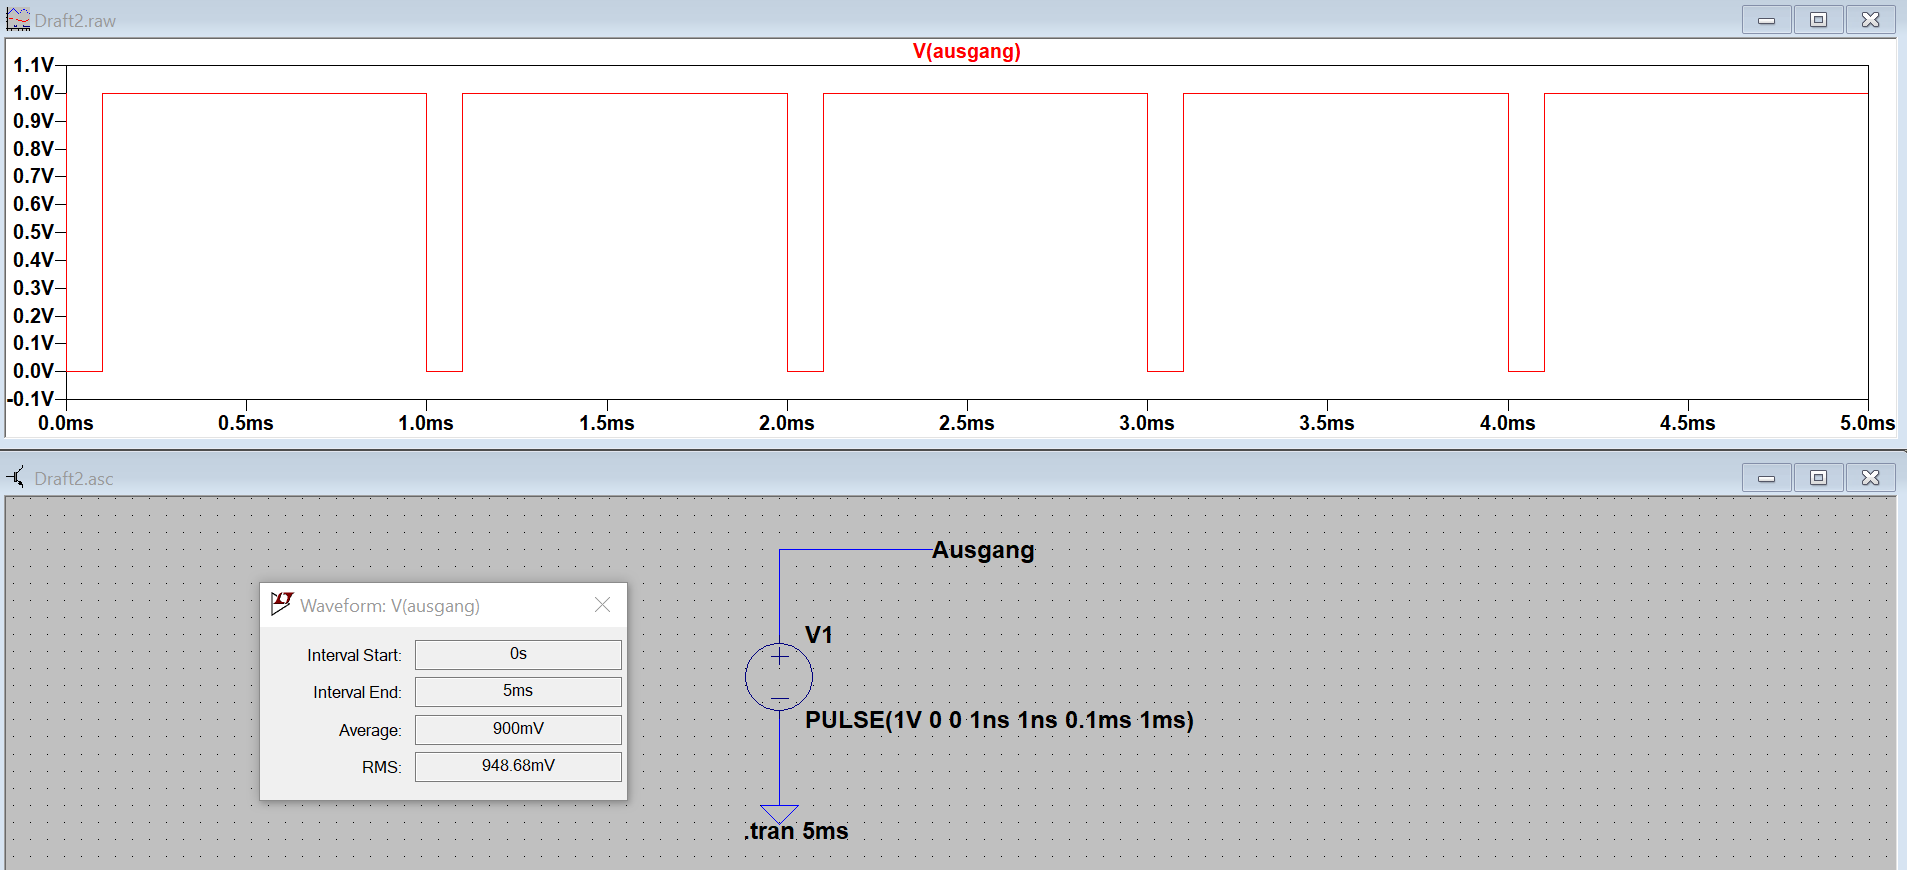
\includegraphics[scale=0.5]{214.PNG}
\caption{Unsymmetrisches Rechtecksignal mit $\^{U}=1V$, $T_{on}=0,1 ms$ und $f=1ms$}
\label{fig: unsymRechtecksignal}
\end{figure}

\subsection{Dreiecksignal}
Damit bei der Simulation mit LTSpice ein Dreiecksignal herauskommt, werden die Werte für $T_{rise}$, $T_{fall}$ und $T_{on}$ angepasst. 
$$T_{rise}=0.5ms$$
$$T_{fall}=0.5ms$$
$$T_{on}=0ms$$
Durch das einfügen der restlichen Werte \fref{fig: Dreiecksignal}, ergibt sich folgende LTSpice Simulation und Graph.
\begin{figure}[ht!]
\centering
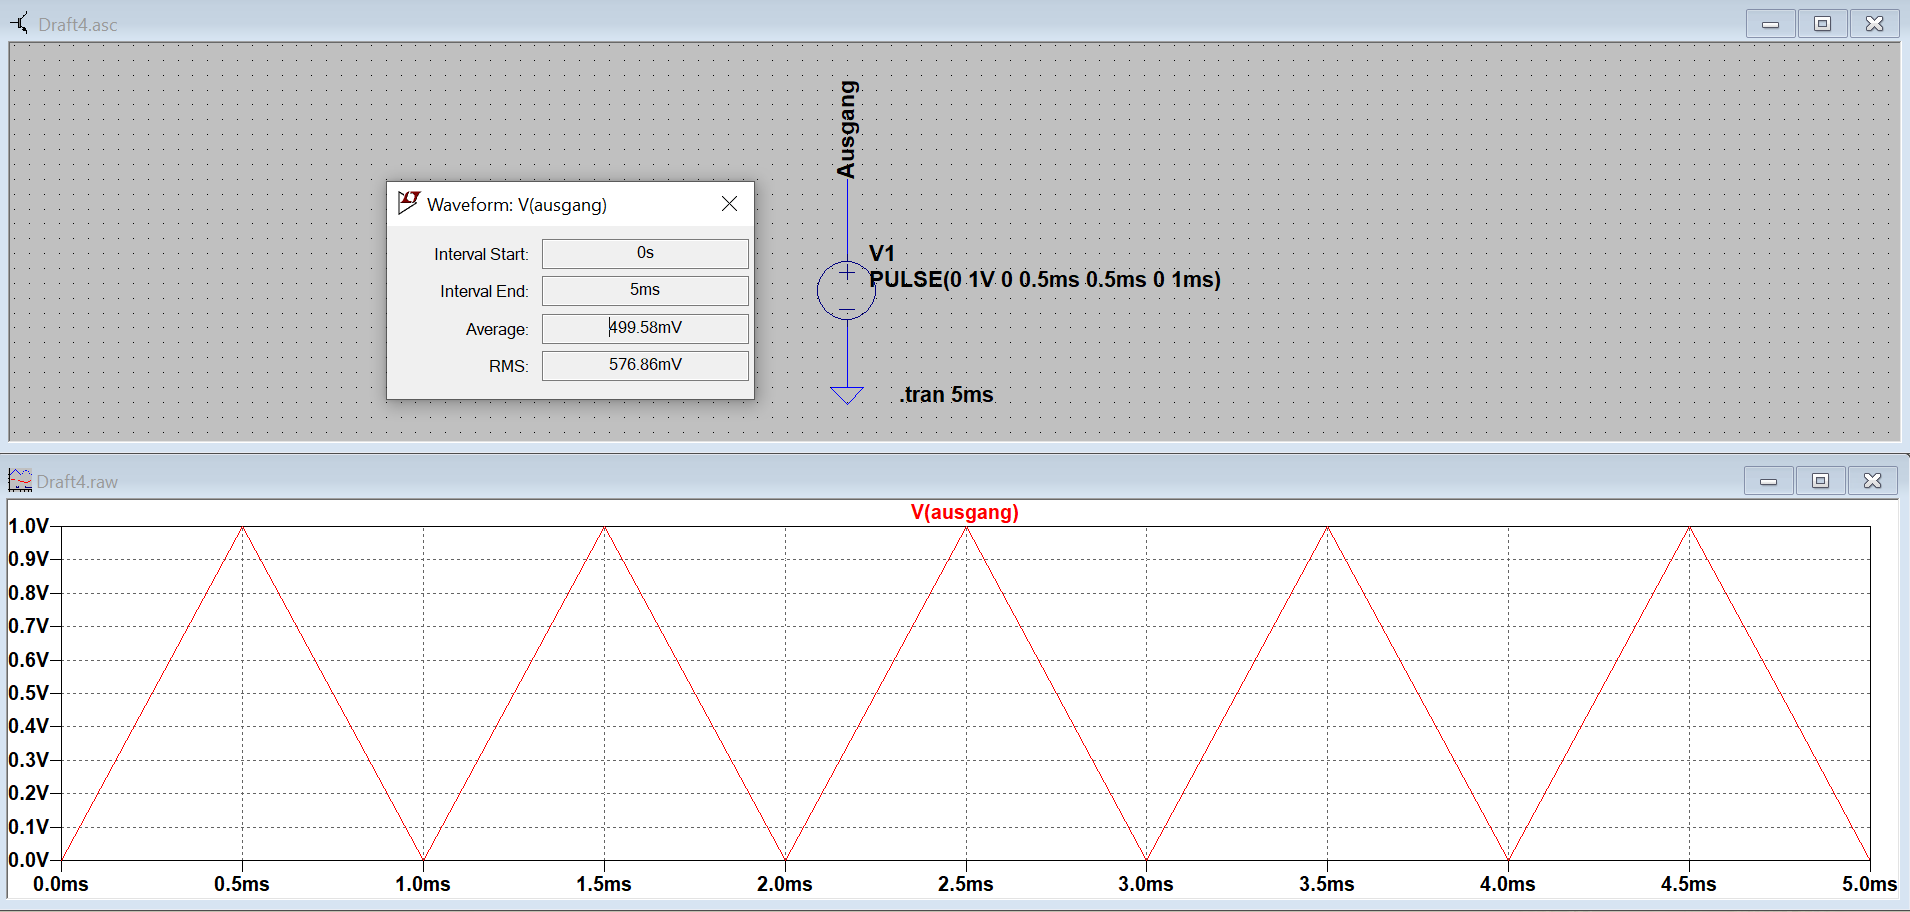
\includegraphics[scale=0.5]{215.PNG}
\caption{Dreiecksignal mit $\^{U}=1V$, $T=1ms$ }
\label{fig: Dreiecksignal}
\end{figure}
\newpage
\subsection{Sägezahnsignal}
Damit bei der Simulation mit LTSpice ein Dreiecksignal herauskommt, werden die Werte für $T_{rise}$, $T_{fall}$ und $T_{on}$ angepasst. 
$$T_{rise}=0.5ms$$
$$T_{fall}=1ns$$
$$T_{on}=0ms$$
Durch das einfügen der restlichen Werte \fref{fig: Sägezahnsignal}, ergibt sich folgende LTSpice Simulation und Graph.

\begin{figure}[ht!]
\centering
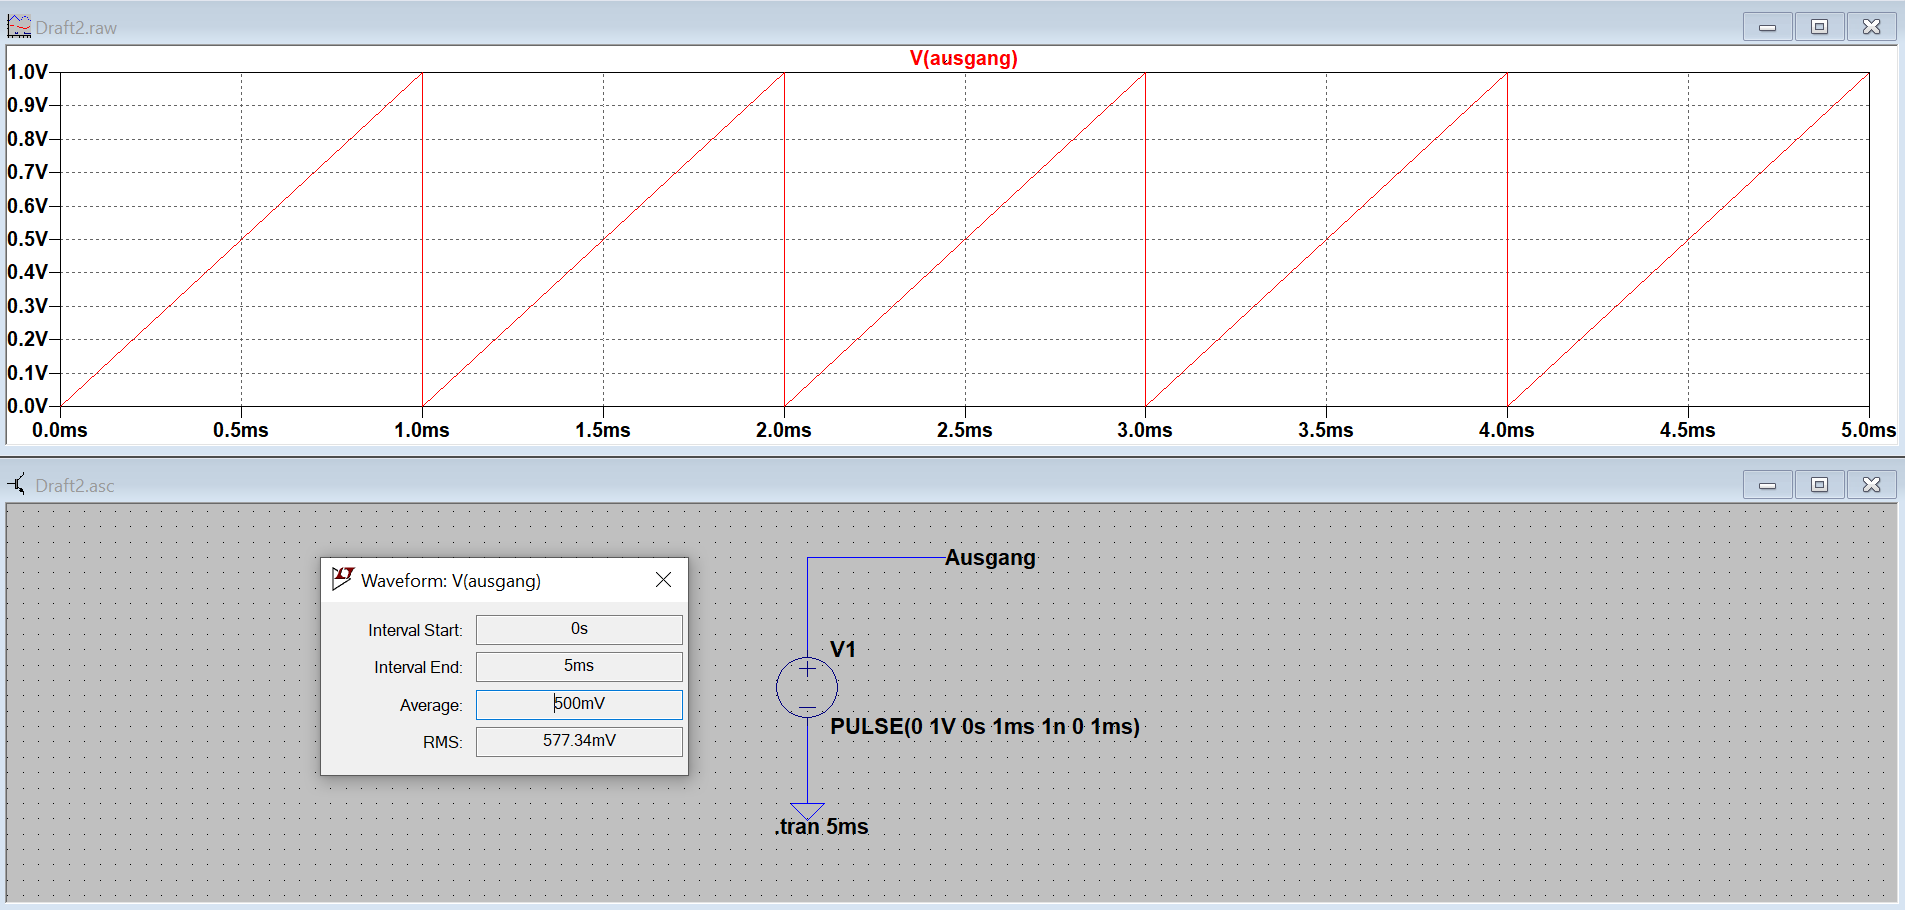
\includegraphics[scale=0.5]{216.PNG}
\caption{Sägezahnsignal mit $\^{U}=1V$, $T=1ms$}
\label{fig: Sägezahnsignal}
\end{figure}



Die von Hand ermittelten Effektivwerte (siehe Abschnitt 1.3) werden im Folgenden mit den Werten aus der Simulation verglichen. Die simulierten Effektivwerte sind auf den einzelnen Abbildungen \ref{fig: Signalquelle} bis \ref{fig: Sägezahnsignal} in den kleinen Kästchen unter RMS zu finden.
\begin{table}[ht!]
\centering
\caption{Wertetabelle für die Effektivwerte}
\label{fig: Effektivwerte}
\begin{tabular}{|c|c|c|} \hline
Signal & simulierte Effektivwerte & berechnete Effektiverte\\ \hline
Gleischspannungsquelle & 1V & 1V\\ \hline
Sinussignal & 707,19mV & 707mV\\ \hline
Symmetrisches Rechtecksignal & 707,11mV & 1V\\ \hline
Unsymmetrisches Rechtecksignal & 948,68mV & 1V\\ \hline
Dreiecksignal & 576,86mV & 578mV\\ \hline
Sägezahnsignal & 577,34mV & 578mV\\ \hline

\end{tabular}
\end{table}

Den Wert für das Sinussignal wurde in 1.3.1 Formel (1.9) berechnet. Der Wert für die Rechtecksignale sind in 1.3.2 Formel (1.17) und für die Dreiecksignale  in 1.3.3 Formel (1.26) zu finden. In Tab. \ref{fig: Effektivwerte} sind diese nochmal nebeneinander gestellt. Beim Vergleichen der Effektivwerte durch Berechnen und durch die Simulation ist direkt zu sehen, dass es dort kleine Unterschiede gibt. Bei dem Sinussignal und dem Dreiecksignal sind die Werte annäherungsweise gleich. Jedoch gibt es bei den Rechtecksignalen Unterschiede zwischen den Effektivwerten. Der des unsymmetrischen Dreiecksignals ist noch annäherungsweise an den errechneten 1V dran, der Effektivwert des symmetrischen Rechtecksignals hat jedoch einen Unterschied von fast 300mV. Dieser Wert passt eher zu dem berechneten Effektivwert des Sinussignals.

\newpage


\section{Spannungsteiler}
\subsection{Unbelasteter Spannungsteiler}
\begin{figure}[h!]
\centering
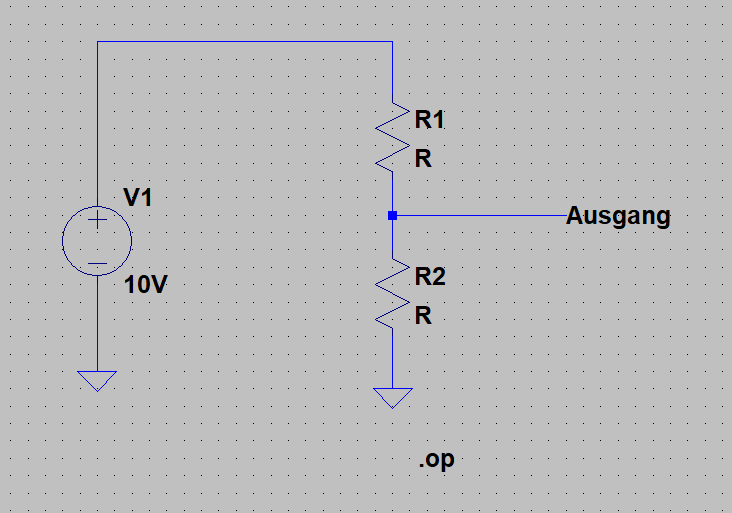
\includegraphics[scale=1]{221.PNG}
\caption{Unbelasteter Spannungsteiler}
\label{fig: Unbelasteter Spannungsteiler}
\end{figure}
Beim unbelasteten Spannungsteiler \fref{fig: Unbelasteter Spannungsteiler} werden jetzt die einzelnen Werte für $R_1$ und $R_2$ verändert und in die Schaltung eingegeben.

\begin{table}[h!]
\centering
\caption{Wertetabelle für den unbelasteten Spannungsteiler }
\label{fig: unbelasteter Spannungsteiler}
\begin{tabular}{|c|c|c|c|} \hline
$R_1$ in $\Omega$ & $R_2$ in $\Omega$ & $V_{aus}$ Simulation in V & $V_{aus}$ Spannungsteilerformel in V\\ \hline
$4,7k$ & $2,2k$ & 3,18841 & 3,18841\\ \hline
$47k$ & $22k$ & 3,18841 & 3,18841\\ \hline
$470k$ & $220k$ & 3,18841 & 3,18841\\ \hline
$4,7M$ & $2,2M$ & 3,18841 & 3,18841\\ \hline
$47M$ & $22M$ & 3,18841 & 3,18841\\ \hline

\end{tabular}
\end{table}

Mit der Spannungsteilerformel 
\begin{equation}
U_{aus}=U_{ges}\cdot \frac{R_2}{R_1+R_2}
\end{equation}
wird die Spannung am Ausgang von Hand berechnet. Dabei ist $U_{ges}=10V$, die Werte für $R_1$ und $R_2$ sind aus der Tabelle \ref{fig: unbelasteter Spannungsteiler} ablesbar.
Die Ergebnisse der Simulation und die Ergebnisse aus der Spannungsteilerformel sind identisch. Desweiteren sind die Ergebnisse für die verschiedenen Werte von $R_1$ und $R_2$ gleich, da diese Vielfache voneinander sind und sich somit die erhöhten Werte ausgleichen.

\subsection{Belasteter Spannungsteiler}
Der belastete Spannungsteiler ist wie der unbelastete Spannungsteiler aufgebaut, jedoch wird an den Ausgang ein Innenwiderstand von $R_3=10M\Omega$ dazugeschaltet. Dies ist in Abb.\ref{fig: bel.Spannungsteiler} veranschaulicht.
\begin{figure}[h!]
\centering
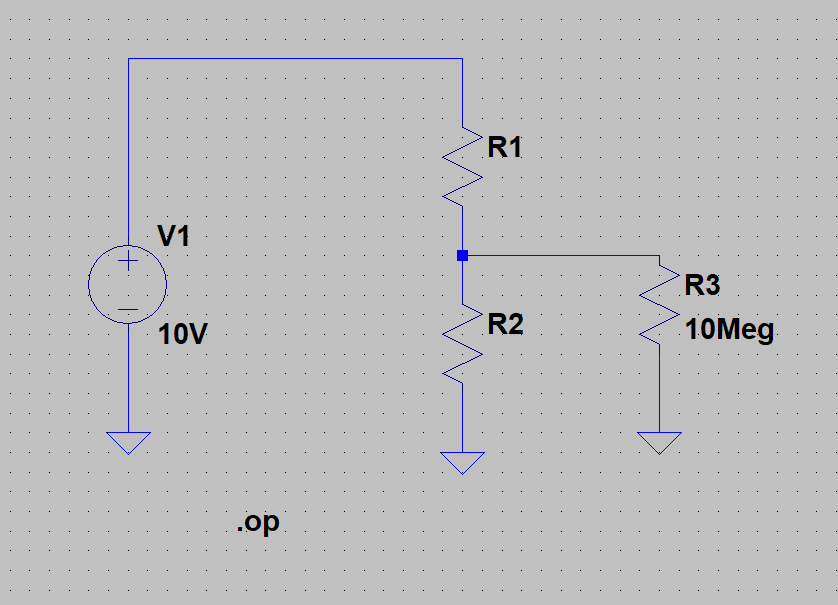
\includegraphics[scale=1]{222.PNG}
\caption{Belasteter Spannungsteiler}
\label{fig: bel.Spannungsteiler}
\end{figure}

\begin{table}[h!]
\centering
\caption{Wertetabelle für den unbelasteten Spannungsteiler }
\label{fig: belasteter Spannungsteiler}
\begin{tabular}{|c|c|c|} \hline
$R_1$ in $\Omega$ & $R_2$ in $\Omega$ & $V_{aus}$ Simulation in V \\ \hline
$4,7k$ & $2,2k$ & 3.18793\\ \hline
$47k$ & $22k$ & 3.18363\\ \hline
$470k$ & $220k$ & 3.14133\\ \hline
$4,7M$ & $2,2M$ & 2.77288\\ \hline
$47M$ & $22M$ & 1.2761\\ \hline

\end{tabular}
\end{table}

Beim Vergleichen der Ausgangsspannung $V_{aus}$ der Simulation (siehe Tab.~\ref{fig: belasteter Spannungsteiler} und~\ref{fig: unbelasteter Spannungsteiler})fällt auf das die Werte voneinander abweichen. Das liegt daran, das ein nicht variabler Widerstand $R_3=10M\Omega$ (Innenwiderstand des Voltmeters) parallel zu $R_2$ dazugeschaltet ist. Da dieser immer den gleichen Wert besitzt, jedoch die Werte für $R_1$ und $R_2$ steigen, verändert sich auch die Spannung am Ausgang. Dies  ist auch an der Formel für einen belasteten Spannungsteiler zu sehen.
\begin{equation}
U_{aus}=U_{ges}\cdot \frac{R_2||R_3}{R_1+(R_2||R_3)}
\end{equation}
Hier wird der Widerstand $R_3$ parallel zu $R_2$ geschaltet und  mit dem festen Wert für $R_3$ gerechnet. Dadurch sinkt die Spannung bei höheren Widerstandswerten von $R_1$ und $R_2$.

\section{Potentiometer}
\begin{figure}[h!]
\centering
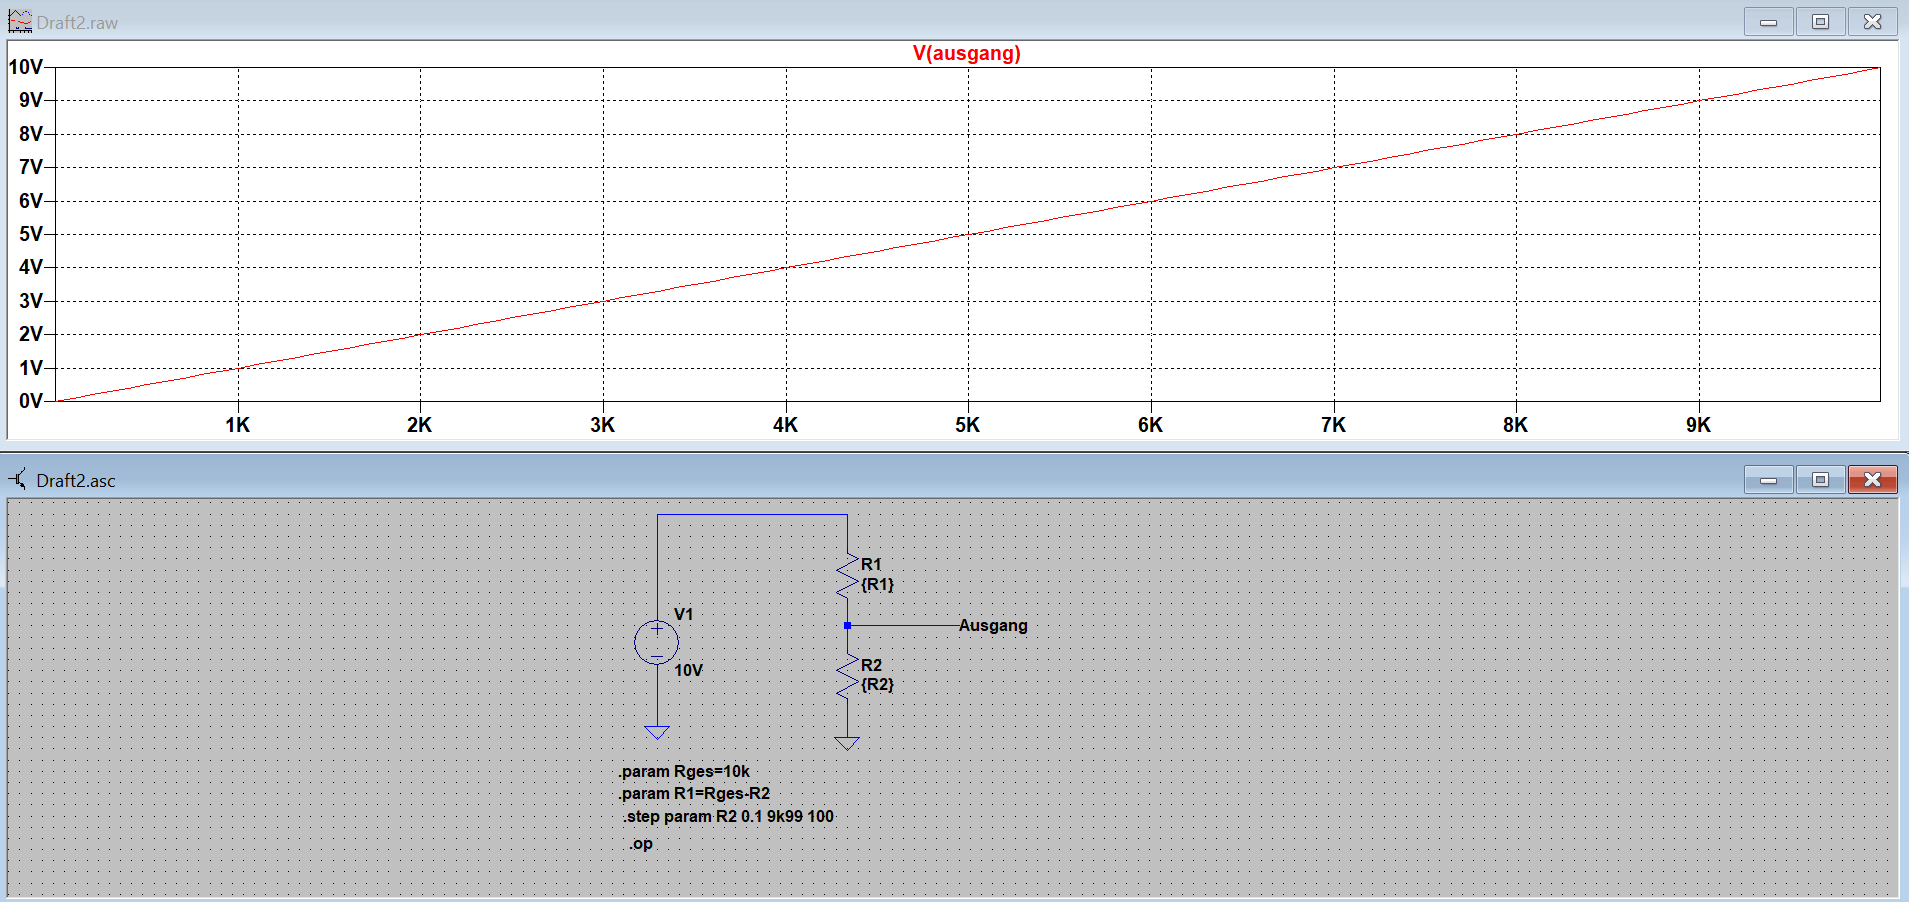
\includegraphics[scale=0.5]{23.PNG}
\caption{Darstellung eines Potentiometers}
\label{fig: Potentiometer}
\end{figure}

Die Schaltung in Abb.~\ref{fig: Potentiometer} sieht aus wie die Abb.~\ref{fig: Unbelasteter Spannungsteiler} eines unbelasteten Spannungsteilers. Jedoch ist beim Potentiometer der Widerstand $R_1$ vom Widerstand $R_2$ abhängig.
\begin{equation}
R_1=R_{ges}-R_2
\end{equation}
Die Werte von $R_2$ ändern sich dabei in $100\Omega$ Schritten im Intervall von $0.1\Omega$ bis $9k99\Omega$, unter der Bedingung:
$$0\Omega \leq R_2\leq R_{ges}$$
Die Simulation beginnt mit $0.1\Omega$ und endet mit $9k99\Omega$ damit $R_1$ nicht $0\Omega$ wird.\\
Im Graphen \fref{fig: Potentiometer} ist zu sehen, das mit steigendem $R_2$ auch die Ausgangsspannung $V_{aus}$ steigt.







